\chapter{Estado del Arte}
En este capítulo presentaremos de manera resumida el trabajo realizado sobre el estado del arte de la recolección de datos de dispositivos móviles. En la última sección profundizaremos su estudio tomando el caso particular de la plataforma Android. En \cite{estadoDelArte} se encuentra el trabajo completo en caso que se desee profundizar en los temas a ver y otros relacionados.

Los temas que no se encuentran directamente relacionados con el presente trabajo fueron omitido del resumen. Entre ellos podemos destacar: SIM cards, redes inalámbricas, tecnologías de almacenamiento flash, formatos de almacenamiento de los datos extraídos, aspectos del almacenamiento de dispositivos Android (en particular, particiones y filesystems habitualmente utilizados en Android), formas de obtener root en dispositivos Android y finalmente el lenguaje DFXML. La mayor parte de los temas mencionados se encuentran íntimamente ligados a lo que conoceremos en la sección \ref{tiposDeMetodosExtraccion} como extracciones físicas, las cuales no forman parte del alcance de nuestro trabajo.

\section{Características de los dispositivos móviles}
Empezaremos por conocer los aspectos fundamentales de este tipo de dispositivos que serán nuestro objeto de estudio. Entender sus características particulares es de suma importancia si pretendemos conocer cómo extraer información de los mismos y entender qué consecuencias tienen nuestras acciones a lo largo de este proceso.

En el área forense, contamos con un desarrollo del conocimiento sobre computadoras personales (PC) muy avanzado. El mismo ha sido posible debido a que si bien en las últimas décadas las capacidades de las PC han estado en constante incremento, las bases de su funcionamiento e interfaces brindadas no han presentado cambios radicales. Esto ha permitido que hoy en día en las PC, al utilizar determinadas metodologías y procedimientos, podamos contar con ciertas garantías sobre los datos extraídos que resultan muy importantes del punto de vista forense.

Las PC son los sistemas informáticos que presentan una mayor semejanza a los dispositivos móviles de hoy en día, debido a la gran cantidad de aspectos que comparten. Por lo tanto, resulta razonable que intentemos aplicar el conocimiento con el que contamos en el área forense sobre las PC, también a los dispositivos móviles. Esto es posible en ciertos aspectos en los que comparten las mismas características con las PC. Sin embargo, veremos que los dispositivos móviles presentan una serie de características muy diferentes, las cuales implican que a menudo no sea posible aplicar las mismas técnicas y debamos buscar nuevas alternativas.

Además de introducir nuevos desafíos desde el punto de vista forense, los dispositivos móviles también brindan nuevas oportunidades al contar con ciertos tipos de información a los cuales no estábamos acostumbrados a encontrar en las PC.

\subsection{Aspectos de hardware}
La cantidad de modelos de dispositivos móviles que existen y su variedad están en continuo aumento. Si consideramos únicamente aquellos dispositivos móviles que corren el sistema operativo Android (el más popular a nivel mundial en este momento \cite{gartnerSales}), podemos observar que a julio de 2013 existían más de 10,000 modelos distintos \cite{androidFragment}.

¿Por qué resulta relevante considerar la inmensa cantidad de modelos de dispositivos móviles que existen, si después de todo, podemos observar que en el terreno de las PC también existe una gran variedad de modelos y sin embargo las herramientas forenses con las que contamos hoy en día no presentan mayores dificultades en soportar esta diversidad?

Resulta que los dispositivos móviles presentan, en la actualidad, una particularidad muy importante que hace que la gran diversidad de modelos sea un hecho relevante. Se trata de que presentan una gran variedad de interfaces de hardware, incluso entre modelos de un mismo fabricante. Esto se ve acentuado por el hecho de que muy a menudo los dispositivos móviles cuentan con hardware especializado. Esta diversidad de interfaces se extiende y probablemente es más visible al público en general al observar la cantidad de conectores de cables de poder y datos que existen para dispositivos móviles. La Unión Europea incluso intentó impulsar regulaciones con el objetivo de obligar a los fabricantes de estos dispositivos a adoptar un estándar único para los conectores de teléfonos celulares \cite{iphoneChargeConn}.

La diferencia a apreciar en la industria de las PC es que el hardware es diseñado con una visión modular para proveer compatibilidad con otras piezas de hardware construidas potencialmente por otros fabricantes. Por ejemplo, en caso de querer acceder a los datos de un disco duro de un PC, contamos con un conjunto de interfaces estándar muy limitado en la industria (IDE, SATA, SCSI).

Si consideramos ahora a los dispositivos móviles, vemos que proveer interoperabilidad entre componentes de hardware de diversos fabricantes no es un objetivo que suelen tener en mente los fabricantes a la hora de diseñar un nuevo dispositivo. Frecuentemente priorizan el poder contar con un diseño compacto, muchas veces soldando los componentes directamente o diseñando chips que integran varias funciones con el objetivo de disminuir el espacio. Esto se evidencia en las arquitecturas SoC (System on a Chip), populares en el mundo móvil. Muchos dispositivos hoy en día vienen incluso con su batería soldada al PCB por esta misma razón.

Mientras en la industria la tendencia de dispositivos móviles con diseños monolíticos se acentúa, un grupo de investigación de Google (Advanced Technology and Projects group) ha tenido la iniciativa, en estos últimos años, de formar la base para contar con dispositivos móviles modulares. Bajo el nombre de \enquote*{Project Ara}, proponen una plataforma que brinde el esqueleto mínimo necesario de interfaces estándar con el objetivo de permitir que fabricantes de diversos tipos de piezas de hardware de dispositivos móviles (como cámara, radio, batería, almacenamiento, etc) puedan diseñarlas de forma que interoperen con facilidad con componentes de otros fabricantes. El usuario del dispositivo entonces tendría la libertad de escoger componentes de diferentes fabricantes según sus necesidades y armar su dispositivo a medida. El proyecto se encuentra en una etapa temprana con prototipos avanzados e interés de varios fabricantes \cite{projectAra}.

Es interesante contemplar por un instante esta iniciativa ya que su éxito podría tener una repercusión significativa en el proceso de adquisición de datos. El hecho de contar con interfaces estándar de hardware podría facilitar en gran medida el proceso. Además, brindaría la habilidad de poder remover físicamente los módulos de hardware con facilidad. Esta última es una diferencia notoria que presentan hoy en día los dispositivos móviles. En particular, cuando consideramos el acceso a datos almacenados, a diferencia de las PC, la unidad de almacenamiento principal se encuentra soldada al PCB del dispositivo. La única forma de remover dicha unidad es mediante técnicas de \enquote*{chip off} como veremos más adelante en la sección \ref{tiposDeMetodosExtraccion}. La excepción a esto son las tarjetas de expansión (SD cards), las cuales se encuentran presentes en muchos modelos. Veremos más adelante que si bien son una fuente de información importante, los datos más sensibles suelen estar en el almacenamiento principal.

\subsection{Aspectos de software}
En esta sección nuestra intención es ver en más detalle los aspectos que caracterizan al software de los dispositivos móviles.

\subsubsection{Sistema operativo}
Hoy en día, todos los sistemas operativos para dispositivos móviles cuentan con capacidades comparables a los tradicionales sistema operativos de PC. Sin embargo, además de presentar grandes cambios en cuanto al diseño de interacción con el usuario, estos sistemas también presentan varios aspectos técnicos importantes que los diferencian de los sistemas anteriores. Veamos algunos de estos aspectos que son de interés:

\begin{enumerate}
\item Uso eficiente de los recursos limitados con los que cuentan.
    \begin{itemize}
    \item \textbf{Poder de procesamiento}: Si bien los dispositivos móviles cada vez cuentan con un mayor poder de procesamiento, la brecha entre el procesamiento con el que cuentan los PCs hoy en día aún es considerable.
    \item \textbf{Almacenamiento}: De forma similar, la capacidad de almacenamiento ha aumentado considerablemente, pero es significativamente menor con la que podemos contar en las PCs, por lo cual tanto aplicaciones como sistema operativo debe hacer un uso eficiente del mismo.
    \item \textbf{Batería}: El ritmo con que avanza la tecnología informática no ha tenido su contrapartida en la tecnología de las baterías. La duración de las mismas no ha aumentado considerablemente. Por lo tanto, el mismo pasa a ser un recurso de mayor relevancia. Para aumentar la duración de la batería se debe intentar ser lo más eficiente posible con todos los recursos del dispositivo en general. Desde el punto de vista del software, esto quiere decir tener mecanismos dentro del sistema operativo como pueden ser disminuir el brillo de la pantalla en ciertas situaciones, matar procesos que hagan uso extenso de los recursos, etc. También implica que los desarrolladores de software deben tener especial cuidado al implementar funcionalidades en sus aplicaciones.
    \end{itemize}
\item Los sistemas operativos móviles introducen varios conceptos de seguridad importantes a sus modelo de seguridad con respecto a los disponibles por defecto en sistemas operativos de PC. Veamos dos muy importantes que se encuentran en los dos sistemas más populares (Android e iOS):
    \begin{itemize}
    \item \textbf{Sandboxing de aplicaciones}: El sistema operativo encapsula a cada aplicación imponiendo una capa a través de la cual la aplicación debe interactuar con el sistema operativo pasando controles antes de acceder a recursos fuera de la misma.
    \item \textbf{Control de acceso a recursos}: Establecen un fuerte control de acceso a recursos basado en permisos. Mediante el mismo buscan comunicar de forma clara al usuario los recursos a los cuales tiene acceso cada aplicación.
    \end{itemize}
\item El ciclo de liberación de versiones de los sistemas operativos móviles es considerablemente más rápido que al que estábamos acostumbrados para sistemas operativos de PC. iOS tiene un promedio de una nueva versión por año \cite{historyOfiOs} mientras que para Android el promedio es menor a un año \cite{androidVersionHistory}. En los sistemas operativos de escritorio el promedio de tiempo entre nuevas versiones rondaba los cuatro años \cite{WindowsHistory}.
\item Por último, como hemos visto, existe una mayor diversidad de sistemas operativos y cambios en las cuotas de mercado de los mismos que en la industria de las PC. Hasta hace unos años, se dió una competencia muy intensa entre varios contendientes con el fin de capturar el mercado. En ese período surgieron muchos sistemas operativos móviles. Hoy en día tenemos dos claros vencedores: Android e iOS \cite{gartnerSales}. De todas formas, continúan surgiendo sistemas operativos móviles como es el caso de Windows Phone (de Microsoft), Tizen (de Samsung), Firefox OS (de Mozilla) y más. Por otro lado, otros que tuvieron gran participación del mercado en el pasado reciente como Blackberry OS, Symbian OS, etc han ido desapareciendo lentamente. Estos cambios en un lapso tan corto le da un aspecto de gran dinamismo a la industria de los dispositivos móviles. Para herramientas que dependen de estas plataformas, esto significa que las mismas en general deben estar en constante actualización.
\end{enumerate}

\subsubsection{Aplicaciones}
Empecemos por recordar que la distribución de aplicaciones en PC tradicionalmente se ha dado de forma descentralizada y los controles que se realizan antes de instalar una aplicación de escritorio suelen ser mínimos por parte del sistema operativo. Veamos cómo el ecosistema de aplicaciones que existe en el mundo móvil es notoriamente distinto.

En el modelo utilizado usualmente por las plataformas móviles se cuenta con una tienda virtual que centraliza el descubrimiento y distribución de aplicaciones. Esto además viene acompañado de un mecanismo que facilita al usuario la instalación y actualización de las mismas. Esta capacidad centralizada le brinda varias ventajas importantes a la organización responsable de la plataforma.

Por un lado, tiene la capacidad de controlar varios aspectos del proceso, entre ellos, cómo los usuarios descubren las aplicaciones, qué tipo de contenido consideran apropiado distribuir, para cuáles regiones geográficas desean que esté disponible cierto contenido, y muchos más. Además, pueden imponer ciertos requerimientos de calidad sobre las aplicaciones.

Por otro lado, tiene la capacidad de implantar mecanismos que le permitan mitigar la distribución de malware y reducir de esta forma significativamente el impacto en los usuarios de la plataforma.

\section{Diversidad de los tipos de datos}
A pesar de las dificultades que suelen presentar los dispositivos móviles a la hora de extraer datos, estos son una excelente fuente de datos ya que cuentan con una gran cantidad de información, mucha de la cual no solemos encontrar en otros tipos de dispositivos como PCs. 

Su naturaleza personal hace que podamos establecer una relación de uno a uno entre el dispositivo y su propietario. Esto facilita la atribución de acciones a un individuo. En investigaciones forenses dicha relación resulta clave al permitir establecer la última milla de evidencia que la relaciona a un individuo \cite{chapter20}.

Hoy en día ya no contamos con un conjunto de tipos de datos finitos y previsibles como era usual al examinar feature phones los cuales contaban con unos pocos tipos de datos como contactos, mensajes, fechas de calendario, etc. Mediante el modelo adoptado por las plataformas móviles, los dispositivos cuentan con acceso de forma muy sencilla a una inmensa cantidad de aplicaciones para una gran diversidad de usos. Esto hace que podamos llegar a encontrarnos con tipos de datos de toda índole.

De esta forma, tendremos que estar preparados para enfrentarnos a una gran diversidad de tipos de datos. Con el fin de tener una noción de los tipos de datos con los que vamos a trabajar, veamos un conjunto representativo de las grandes categorías de los tipos de datos encontrados en dispositivos móviles que suelen ser de interés en investigaciones forenses:

\begin{itemize}
\item Telefonía
\item PIM (Personal Information Management)
\item Mensajería
\item Redes sociales
\item Geolocalización
\item Metadatos
\item Sistema operativo
\item Servicio celular
\end{itemize}

En el documento completo de Estado del Arte en \cite{estadoDelArte}, el lector podrá encontrar varios ejemplos de tipos de datos para cada categoría y ejemplos de los usos que se le pueden dar en el contexto de una investigación forense.

\section{Tipos de métodos de extracción}
\label{tiposDeMetodosExtraccion}

A la hora de extraer los datos de un dispositivo móvil es necesario tener en cuenta las características del método de extracción a utilizar. Estas características hacen referencia tanto a las capacidades de los métodos a la hora de obtener los datos como a las consecuencias que los mismos tengan sobre el dispositivo \cite{cellphoneevidence}.

En la siguiente figura se puede ver los distintos tipos de métodos de extracción:

\begin{figure}[H]
    \begin{center}
        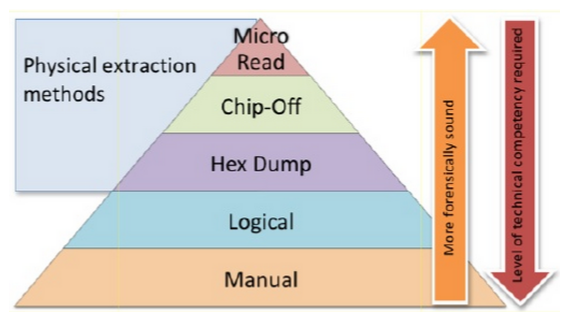
\includegraphics[width=\textwidth]{figures/extraction_methods_types}
        \caption{Tipos de métodos de extracción}
    \end{center}
\end{figure}

A medida que nos movemos hacia la cima de la pirámide, los métodos:

\begin{itemize}
\item Resultan más limpios desde el punto de vista forense.
\item Requieren de utilizar herramientas más caras.
\item Requieren mayor conocimiento técnico.
\item Exigen más tiempo para analizar los datos extraídos.
\item Requieren más entrenamiento.
\item Son más invasivos.
\end{itemize}

Comenzando por la base de la pirámide, los métodos \emph{manuales} requieren interactuar con el dispositivo utilizando el teclado o pantalla táctil del mismo para obtener los datos. Esto hace que este tipo de métodos sea soportado por una gran cantidad de dispositivos. Dado que la interacción con el dispositivo se da a través del sistema operativo, únicamente se pueden obtener datos que estén disponibles a través del mismo \cite{chapter20}.

En el segundo nivel se encuentran los métodos de extracción \emph{lógicos}, los cuales consisten en conectar el dispositivo a una PC y utilizar algún protocolo de intercambio de datos para obtener los datos del dispositivo. Al igual que con los métodos manuales, los únicos datos que se pueden obtener son los accesibles a través del sistema operativo. Son métodos rápidos, automatizables y la interpretación de los datos obtenidos cuenta con las abstracciones del sistema operativo.

En el tercer nivel tenemos los métodos de extracción \emph{físicos}. Estos consisten en copiar de forma parcial o total los datos del dispositivo en su forma bruta (raw data). A diferencia de los métodos manuales y lógicos, los métodos físicos no interactúan con el sistema operativo del dispositivo. Debido a esto, se puede obtener la totalidad de los datos del dispositivo (incluyendo datos borrados), pero hay que tener en cuenta que estos datos deberán ser interpretados.

En el cuarto nivel se encuentran los métodos conocidos como \emph{chip-off}. Como lo dice su nombre, estos métodos consisten en remover físicamente el chip de memoria del dispositivo, y luego (utilizando equipos especializados) realizar la lectura del contenido del chip de forma directa. Al igual que los métodos del nivel anterior, estos métodos permiten obtener la totalidad de los datos del dispositivo. Los aspectos negativos más importantes son el hecho de que el dispositivo queda inoperante y los datos obtenidos deben ser interpretados.

En el último nivel se encuentran los métodos \emph{micro read}. En estos métodos se utilizan microscopios poderosos para ver el estado de la memoria del dispositivo, siendo los mismos los más difíciles y caros de llevar a cabo.

\section{Lenguajes de representación de los datos}
Tras tener los datos extraídos, comienza la tarea de organizar la información relevante que encontremos en los mismos. Para esto, se suelen utilizar lenguajes mediante los cuales podamos representar los datos relevantes que fueron adquiridos e información sobre el proceso utilizado para extraerlos.

De esta forma, estos lenguajes nos permiten expresar y compartir datos relevantes de una investigación. Esto puede resultar de inmensa importancia cuando se requiere trabajar con varios equipos dado que facilita en gran medida la colaboración. Además, nos permite automatizar procesos, y en la medida que el lenguaje adquiera adopción, su interoperabilidad entre herramientas resultará más sencilla.

Es importante que tengamos en cuenta que la elección del lenguaje para representar los datos examinados limitará las herramientas con las que podremos trabajar con facilidad. Uno de los inconvenientes presentes hoy en día en la comunidad forense es el hecho de que cada herramienta comercial utiliza sus propios formatos propietarios y esto hace que la interoperabilidad entre herramientas sea difícil. Por esto, resultan de gran importancia las iniciativas que están surgiendo de formatos abiertos y los esfuerzos de estandarización \cite{oasisAdAutomaged}.

En los últimos años han surgido varios lenguajes de representación de datos de evidencia forense que son interesantes. En particular, nosotros consideramos dos (CybOX y DFXML) para su uso en el trabajo. Ambos son lenguajes abiertos y que poseen un desarrollo activo del mismo y sus herramientas.

En \cite{storageAndExchange} se realiza un estudio comparativo de las diversas alternativas de lenguajes de intercambio que se podían encontrar en 2010. Entre ellos, se describen los siguientes dos: DEX (Digital Evidence Exchange) \cite{DexDigitalEvidence} y XIRAF \cite{DexXmlBased}, los cuales plantean ideas interesantes pero los que no llegamos a considerar debido a que en el primer caso el lenguaje no cuenta con un desarrollo activo desde hace años y en el segundo caso tanto el lenguaje como el framework que lo soporta no se encuentran disponibles públicamente. 

Por lo tanto, nuestras alternativas a considerar fueron DFXML y CybOX. Nos inclinamos por CybOX no sólo debido a la gran comunidad activa que posee, sino también porque permite representar prácticamente todos los datos que permite representar DFXML y por el hecho de que DFXML está diseñado para trabajar únicamente con extracciones físicas. A continuación veremos los aspectos que consideramos importantes conocer sobre CybOX para luego comprender su uso en este trabajo.

\subsection{CybOX}
CybOX \cite{cyboxGitHub} es un lenguaje estructurado para representar lo que se denominan \emph{cyber observables}. Estos son eventos o propiedades con estado que pueden ser observados en el dominio cibernético. El lenguaje no busca satisfacer un caso de uso en particular, sino que intenta ser lo suficientemente flexible para prestar una solución común a un amplio espectro de casos de uso de ciberseguridad que requieran manejar cyber observables.

CybOX soporta un amplio espectro de dominios de ciberseguridad incluyendo caracterización de amenazas, caracterización de malware, manejo operacional de eventos, respuesta de incidentes, intercambio de indicadores de compromiso, digital forensics y más.

De esta forma, vemos que CybOX es utilizado para una gran diversidad de finalidades. En cada una de estas el mismo generalmente es utilizado de forma indirecta, esto es, a través de otro lenguaje que aprovecha su expresividad para describir cyber observables en su dominio.

\subsubsection{¿Qué intenta resolver?}
Podemos considerar tres principios que caracterizan las intenciones del lenguaje \cite{observableExp}:

\begin{enumerate}
\item \textbf{No está dirigido a un caso de uso de ciberseguridad en particular}: La intención es que sea lo suficientemente flexible para ofrecer una solución común para todos los casos de uso de ciberseguridad que requieran la capacidad de trabajar con cyber observables. Por lo tanto, busca principalmente ser una infraestructura para representar esta información, sobre la cual puedan construirse otros estándares y soluciones en cada dominio de trabajo específico.
\item \textbf{Flexibilidad tanto para expresar instancias como potenciales patrones}: También busca ser lo suficientemente flexible para permitir describir tanto instancias de cyber observables de alto grado de fidelidad como patrones más abstractos de potenciales cyber observables.
\item \textbf{Visión de automatización integrada}: Al tener especificado un esquema común y estructurado para los cyber observables, es posible desarrollar la capacidad de automatizar el intercambio de información detallada de los mismos.
\end{enumerate}

\subsubsection{Componentes de CybOX}
CybOX presenta un modelo de datos separado en cuatro componentes:

\textbf{Core}: Consiste en los esquemas CybOX Core y CybOX Common que definen las construcciones básicas del lenguaje (como \emph{Observable} y \emph{Property}) y tipos de datos comunes utilizados por objetos (como \emph{HashType} y \emph{TimeType}).

\textbf{Objects}: Consiste de todos los esquemas de los objetos predefinidos que vienen por defecto con CybOX. Entre estos podemos encontrar Device, File, URI, User Account, etc.

\textbf{Vocabularies}: Consiste en varias listas de valores definidos que suelen resultar útiles para el uso por parte de los objetos. Por ejemplo, \emph{HashNameEnum} contiene una lista de algoritmos de hashing como MD5, SHA256, etc. Es posible también crear uno mismo sus propios vocabularies.

\textbf{Extensions}: Consiste de esquemas externos que utiliza CybOX para representar algún aspecto como puede ser localización geográfica a través de CIQ o describir plataformas a través de CPE.

\subsubsection{¿Por qué y para qué nos sirve?}
El lenguaje es de nuestro interés por las siguientes características que presenta:

\begin{itemize}
\item Su capacidad de representar propiedades con estado, hace que sea posible representar datos obtenidos en una extracción y metadatos de forma estructurada.
\item El dominio de información sobre la cual trabaja incluye al de digital forensics. Muchos de los objetos predefinidos son relevantes a nuestro dominio y esto hace que podamos reutilizarlos.
\item La visión de automatización y las diversas herramientas que proporciona para facilitar su procesamiento es un aspecto clave. Consideramos importante que la información producida en el lenguaje pueda ser utilizada por parte de otras herramientas con facilidad.
\item El hecho de que sea un lenguaje estándar y el mismo sea utilizado por diversas comunidades es también importante. Indica la madurez del mismo y ayuda al soporte del mismo por parte otras herramientas.
\end{itemize}

\subsubsection{Representación de tipos de datos}
Como vimos, un aspecto interesante de CybOX es que el mismo nos brinda un conjunto de objetos predefinidos relevantes para el dominio de digital forensics. En su última versión a la fecha (2.1), podemos observar objetos como File, Email Message, SMS Message, URI, etc que nos permiten representar varios tipos de datos de interés en el contexto del trabajo.

Por otro lado, cabe destacar que también es posible extender el conjunto de objetos que nos permite representar CybOX (esto es, más allá de los predefinidos). En la siguiente sección, veremos cómo podemos utilizar un mecanismo que brinda CybOX para hacer esto.

\subsubsection{Utilizando CustomObject}
El objeto \emph{CustomObject} nos permite especificar objetos que no tienen un schema definido. Esto hace que resulte fácil utilizarlos para representar nuevos objetos pero para esto ambos productor y consumidor deben ponerse de acuerdo en los campos declarados dado que no cuenta con un schema que defina el nombre y tipo de cada uno.

Veamos un ejemplo en el cual tenemos un \emph{CustomObject} \cite{customObject} que representa la contraseña de un documento de Microsoft Office:
\newline

\begin{xml}
<CustomObj:CustomObjectType xsi:type="CustomObj:CustomObjectType" custom_name="example:OfficePassword">
  <cyboxCommon:Custom_Properties>
    <cyboxCommon:Property name="password" 
    description="MS Office encryption password">
      SuP3rS3cr3T!
    </cyboxCommon:Property>
  </cyboxCommon:Custom_Properties>
    <CustomObj:Description>
      This is a string used as a password to protect an Microsoft Office document.
    </CustomObj:Description>
</CustomObj:CustomObjectType>
\end{xml}

\subsubsection{Extensión del lenguaje}
\label{extensionDelLenguaje}
Desde el punto de vista técnico, CybOX es un lenguaje que está basado en XML y se encuentra definido utilizando XML Schema. Esto implica que debemos contar con buen conocimiento de estos lenguajes si deseamos extender CybOX.

Existen varios puntos de extensión del lenguaje CybOX. En particular, los más frecuentes suelen ser la definición de nuevos objetos y vocabularios. Nosotros vamos a concentrarnos en el más interesante para nosotros que es extender el lenguaje mediante la definición de nuevos objetos, dado que nos permitan representar tipos de datos que no son considerados por el lenguaje actualmente.

\textbf{Creando un nuevo objeto de CybOX} \newline
Para crear un nuevo objeto en CybOX es necesario extender el tipo abstracto \emph{ObjectPropertiesType} que se encuentra definido en CybOX Common. Hay dos formas ligeramente distintas de hacer esto:

\begin{itemize}
\item Extender directamente de \emph{ObjectPropertiesType}. Básicamente vamos a estar creando un objeto totalmente nuevo. Esta construcción nos brinda la capacidad de definir las propiedades del objeto.
\item Extender indirectamente de \emph{ObjectPropertiesType}. Esto es, no extender de \emph{ObjectPropertiesType} sino de otro objeto CybOX. Este otro objeto a su vez extiende, ya sea directa o indirectamente, a \emph{ObjectPropertiesType} dado que todos los objetos deben extender a éste.
Esta forma nos permite reutilizar objetos CybOX, evitando duplicar formas de expresar lo mismo y teniendo un modelo de datos más coherente.
Por ejemplo, podemos tener un objeto de tipo \emph{FileObjectType}. Si queremos ser más específicos, podemos optar por un objeto \emph{ImageFileObjectType} que extiende a \emph{FileObjectType} y agrega algunas propiedades como formato de imagen, dimensiones de la imágen, etc.
\end{itemize}

A su vez, resulta importante tener en cuenta los recursos disponibles con los que contamos en CybOX Common y CybOX Vocabularies. En particular, todos los tipos de datos simples que solemos contar en la mayor parte de los lenguajes ya se encuentran definidos (excepto booleano) en CybOX Common. Dentro de CybOX Vocabularies, podemos encontrar varias listas de valores que nos pueden resultar útiles como nombres de algoritmos, estándares de encoding de caracteres, etc.

La documentación de CybOX \cite{cyboxGitHub} provee una guía que describe a grandes rasgos los pasos que debemos tomar cuando vamos a crear un nuevo objeto:

\begin{enumerate}
\item Decidir qué es lo que queremos representar en CybOX.
\item Determinar qué campos/atributos pueden ser utilizados para caracterizar el objeto CybOX.
\item Establecer una correspondencia entre los tipos de datos de dichos campos y los tipos de propiedades disponibles en CybOX.
\item Revisar objetos CybOX existentes para ver si las capacidades que definimos en los pasos anteriores ya no se encuentran soportadas por un objeto existente. Además, identificar objetos CybOX que soporten un subconjunto de las capacidades necesarias, de forma de evaluar extenderlo y cubrir las restantes.
\item Definir un namespace para el objeto.
\item Crear el esquema para el objeto.
\item Agregar documentación al esquema.
\end{enumerate}

\textbf{Ejemplo}
Veamos cómo podemos extender el Device Object de CybOX para que pueda representar un dispositivo más concreto: un teléfono celular. Por lo tanto, además de incluir descripción, fabricante, modelo, número de serie, versión de firmware, etc que ya incluye un Device Object, debemos agregarle IMSI, IMEI y ICCID. Aquí ya hicimos los primeros cuatro pasos.

A continuación debemos escoger un namespace para nuestro nuevo TelephoneDevice Object (\url{http://fing.edu.uy/objects\#TelephoneDeviceObject-2}) y crear un archivo \emph{Telephone\_Device.xsd} que contenga el siguiente esquema:
\newline

\begin{xml}
<xs:schema elementFormDefault="qualified"
  xmlns:xs="http://www.w3.org/2001/XMLSchema"
  xmlns:cyboxCommon="http://cybox.mitre.org/common-2"
  xmlns:DeviceObj="http://cybox.mitre.org/objects#DeviceObject-2"
  xmlns:TelephoneDeviceObj="http://fing.edu.uy/objects#TelephoneDeviceObject-2"
  targetNamespace="http://fing.edu.uy/objects#TelephoneDeviceObject-2"
  version="1.0">
  <xs:import namespace="http://cybox.mitre.org/common-2" schemaLocation="../cybox_common.xsd"/>
  <xs:import namespace="http://cybox.mitre.org/objects#DeviceObject-2" schemaLocation="Device_Object.xsd"/>
  <xs:element name="Telephone_Device" type="DeviceObj:DeviceObjectType"/>

  <xs:complexType name="TelephoneDeviceObjectType">
    <xs:complexContent>
      <xs:extension base="DeviceObj:DeviceObjectType">
        <xs:sequence>
          <xs:element name="IMSI" type="cyboxCommon:StringObjectPropertyType" minOccurs="0"/>
          <xs:element name="IMEI" type="cyboxCommon:StringObjectPropertyType" minOccurs="0"/>
          <xs:element name="ICCID" type="cyboxCommon:StringObjectPropertyType" minOccurs="0"/>
        </xs:sequence>
      </xs:extension>
    </xs:complexContent>
  </xs:complexType>
</xs:schema>
\end{xml}

Si bien es bastante verbosa la representación, lo único que tuvimos que hacer conceptualmente fue extender el objeto Device de CybOX y agregarle las tres propiedades que queríamos (IMSI, IMEI, ICCID) como strings.

Finalmente, para verificar que el esquema sea válido podemos verificarlo con la herramienta \texttt{xmllint} (disponibles en sistemas basados en Unix) de la siguiente forma:
\newline

\begin{bash}
xmllint --noout --dtdvalid http://www.w3.org/2001/XMLSchema.dtd Telephone_Device.xsd
\end{bash}

\section{Plataforma Android}
En esta sección estudiaremos las características más importantes a tener en cuenta para extraer datos de un dispositivo Android. Veremos la arquitectura de la plataforma y el modelo de seguridad impuesto por la misma. Luego, observaremos los datos que podemos encontrar en estos dispositivos y las estructuras en que éstos son almacenados. Finalmente, terminaremos mostrando los mecanismos que podemos utilizar para extraerlos.

\subsection{Arquitectura de la plataforma}
La plataforma Android está diseñada como un stack de componentes de software, en donde se pueden ver 5 secciones, las cuales están divididas en 4 capas \cite{androidArch}.
\newline

\begin{figure}[H]
    \begin{center}
        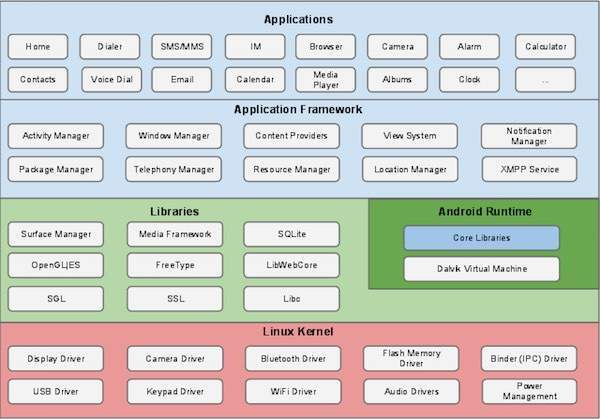
\includegraphics[scale=0.6]{figures/android_architecture}
        \caption{Arquitectura de la plataforma Android}
    \end{center}
\end{figure}

La capa inferior consiste en un kernel Linux modificado, el cual provee una capa de abstracción para interactuar con el hardware. Contiene todos los drivers necesarios para interactuar con los distintos componentes del hardware (cámara, teclado, Wifi, audio, etc).

La segunda capa consta de dos secciones. Por un lado, un conjunto de bibliotecas específicas para cada componente de hardware, las cuales le permiten al dispositivo el manejo de un gran conjunto de datos. Por otro lado, el entorno de ejecución de Android, el cual provee un componente clave para la ejecución de las aplicaciones: \emph{Dalvik Virtual Machine}. Cada aplicación tendrá su propia instancia de Dalvik VM, permitiendo que la aplicación ejecute dentro de un ambiente controlado e independiente. De esta forma, una aplicación no puede interferir indebidamente con otras aplicaciones, con el sistema operativo, ni acceder directamente al hardware del dispositivo.

La tercera capa consta del \emph{Application Framework}, encargado de brindar muchos de los servicios de alto nivel a las aplicaciones a través de clases java, para que los desarrolladores de aplicaciones puedan usarlos en las mismas. Por ejemplo, uno de estos servicios son los \emph{Content Providers}, los cuales son utilizados por las aplicaciones para comunicar datos a otras aplicaciones.

Finalmente, en la cuarta capa se encuentran las aplicaciones instaladas en el dispositivo. Este conjunto de aplicaciones incluye tanto las pre-instaladas como las instaladas por el usuario.

\subsection{Información del sistema}
Como ya vimos, Android fue creado sobre Linux, por lo que estas dos plataformas cuentan con características en común. Una característica muy útil para obtener datos del sistema, son los logs. Existen varios logs de los cuales se pueden obtener datos del sistema, siendo log \emph{dumpsys} el que brinda más información. Para acceder a este log primero es necesario que el dispositivo se encuentre en modo \emph{debug}. Luego, debemos ejecutar el comando \textit{adb shell dumpsys}.

Entre los datos que se pueden encontrar en este log se destacan cuentas sincronizadas, últimas coordenadas GPS conocidas, notificaciones del dispositivo, información del sistema (versiones del kernel, bootloader, etc), información de telefonía (MEID y ICCID) e información sobre el uso del dispositivo (por ejemplo, últimas aplicaciones utilizadas).

\subsection{Información de las aplicaciones}
Las distintas formas de almacenamiento que pueden ser utilizadas por las aplicaciones son las siguientes \cite{androidStrg}:

\begin{itemize}
\item \textbf{SharedPreferences}: Los SharedPreferences son archivos con formato XML, en los cuales el desarrollador de la aplicación puede almacenar un listado de parejas clave- valor de tipos de datos primitivos (booleans, floats, ints, longs y strings). Suelen ser utilizados para almacenar configuraciones de la aplicación, incluyendo los cambios de configuración realizados por el usuario. Estos datos son mantenidos a través de las sesiones del usuario, incluso cuando se cierra la aplicación. 
\item \textbf{SQLite databases}: Este tipo de bases de datos es el más utilizado por la comunidad Android, debido a que su código es Open Source, compacto y toda la base de datos se encuentra en un único archivo. 
\item \textbf{Otros tipos de archivos}: Es posible que las aplicaciones almacenen otros tipos de archivos (por ejemplo video, audio, texto, etc). Estos archivos pueden almacenarse o bien en memoria interna en un directorio que es privado para la aplicación, o bien en memoria externa (esto es, la SD-Card) en un directorio que es accesible por las demás aplicaciones.
\end{itemize}

La estructura de directorios con que cuenta una aplicación en su directorio privado en el almacenamiento de memoria interna es la siguiente:

\begin{itemize}
\item \textbf{databases}: directorio que contiene las bases de datos SQLite manejadas por la aplicación. Además de las bases de datos en sí, se pueden encontrar bases de datos temporales, las cuales son utilizadas por SQLite para realizar rollbacks.
\item \textbf{cache}: directorio utilizado para almacenar archivos temporales. Estos datos pueden ser borrados automáticamente por la aplicación en caso de que no haya espacio suficiente en la memoria interna.
\item \textbf{files}: directorio para almacenar archivos creados por la aplicación cuando la misma desea que los mismos no sean públicos para las demás aplicaciones.
\item \textbf{shared\_prefs}: directorio donde se almacenan los archivos SharedPreferences.
\end{itemize}

Cabe destacar que las aplicaciones también cuentan con la posibilidad de almacenar datos de forma remota a través de internet. Esto a menudo resulta importante cuando las aplicaciones desean evitar almacenar información sensible en el dispositivo.

\subsection{Preparación del dispositivo para la extracción: Rooting}
En el modelo de seguridad que impone Android, el dispositivo viene de fábrica en un estado en el cual el usuario del mismo no tiene acceso directo a gran parte de los datos que se encuentran en el mismo. De esta forma, para acceder a los datos encontrados dentro del área de almacenamiento privada de las aplicaciones o para crear una disk image del dispositivo, debemos hacer lo que se conoce popularmente como \emph{rooting} del dispositivo.

Rooting es el proceso mediante el cual se obtiene root en un dispositivo Android. El mismo se realiza de la misma forma que otros sistemas Linux: explotando una vulnerabilidad. Tras haber obtenido root, es posible modificar el contenido del dispositivo, acceder a zonas protegidas del mismo ó incluso utilizar recursos de hardware sin las restricciones impuestas por el fabricante.

Existen tres tipos de rooting:
\begin{itemize}
\item \textbf{Temporal}: el dispositivo vuelve a sus condiciones normales una vez que es reiniciado.
\item \textbf{Permanente}: se modifican varios archivos del firmware del dispositivo, haciendo que los privilegios se conserven al reiniciar el dispositivo.
\item \textbf{Recovery mode}: se flashea una ROM customizada de la partición de recuperación, mediante la cual se inicia el sistema con privilegios de root.
\end{itemize}

Desde el punto de vista de la extracción de datos, no es necesario realizar un rooteo permanente del dispositivo, ya que un rooting temporal brinda el acceso necesario a las áreas protegidas, y los datos modificados por este proceso volverán a su estado original una vez reiniciado el dispositivo.

Algunas de las consideraciones que se deben tener en cuenta cuando se va a realizar el rooting del dispositivo son \cite{collectmethod}:

\begin{enumerate}
\item Dado que el proceso de rooteo se basa en aprovechar una vulnerabilidad del dispositivo, esta vulnerabilidad depende del modelo y versión de Android del mismo. Por lo tanto, es importante conocer las caracteristicas del mismo antes de realizar el rooteo.
\item Al realizar el rooting del dispositivo se pierden las protecciones del modelo de seguridad de Android, ya que un dispositivo rooteado permite la ejecución de aplicaciones con privilegios totales.
\item Se pueden llegar a modificar áreas del dispositivo en las cuales se guardan datos del usuario.
\end{enumerate}

Sin embargo, a pesar de que existen estos riesgos, el rooting es el proceso que se usa habitualmente si se quieren obtener los datos sensibles encontrados en el dispositivo.

\subsection{Alternativas a rooting}
\label{alternativasRooting}

La primera alternativa es utilizar el comando \emph{adb backup}. El mismo no requiere que se haya hecho el rooting del dispositivo, pero sí requiere que el mismo tenga activada la opción de ADB Debugging, la cual se cambia dentro sus configuraciones. Con este comando es posible realizar un respaldo de los datos internos de las aplicaciones o de la tarjeta SD del dispositivo, y también se puede indicar que se extraiga el apk de las mismas.

Para completar el respaldo con éxito, se requiere intervención por parte del usuario del dispositivo móvil. Al momento de ejecutar el comando desde la consola de la PC, en la pantalla del dispositivo se muestra un diálogo, donde se solicita confirmación.

Los desarrolladores de aplicaciones cuentan con la posibilidad de deshabilitar el backup de datos de su aplicación, esto es, no permitir el respaldo de los datos que la aplicación mantiene en su región de almacenamiento interno privado. Sin embargo, observamos que la mayoría de las aplicaciones suelen tener la opción de respaldo habilitada.

La segunda alternativa es instalar una \emph{CRMI} (Custom Recovery Mode Image). El modo de recuperación de Android fue diseñado para realizar actualizaciones, formatear y realizar operaciones de mantenimiento sobre el dispositivo. Las funcionalidades brindadas por este modo son limitadas, y ninguna de ellas brinda la capacidad de obtener privilegios de root. Sin embargo, mediante la instalación de particiones customizadas de recuperación, se pueden obtener estos privilegios. 
Una vez que se tiene una CRMI, se la flashea sobre la partición de booteo, y se reinicia el dispositivo. Luego de iniciado, se cuenta con privilegios de root, pudiéndose obtener todos los datos deseados. Dado que no es necesario montar la partición de datos del usuario, la copia puede realizarse sin correr el riesgo de que se alteren los datos, incluso datos borrados. Luego de realizar la extracción deseada, se debe volver a flashear la versión original de la partición de booteo \cite{dataintegr}.